\documentclass{beamer}

\title{File Corruption Repair using Reed-Solomon Codes}
\author{Theodor Negrescu}
\date{2025-07-04}

\begin{document}

\frame{\titlepage}

\begin{frame}
\frametitle{Outline}
\tableofcontents
\end{frame}

\section{Introduction}
\begin{frame}
\frametitle{Introduction}
\begin{itemize}
\item
\textbf{Error correction} is an important subject in computer science, relevant for backups, cloud storage, high-reliability systems, and many more applications.
\item
This presentation provides an overview of the theoretical background and implementation details of a utility which repairs file corruption using \textbf{Reed-Solomon codes}.
\item
The utility, named \texttt{rsarc} (Reed-Solomon Archive), is a command-line program written in Rust, available on GitHub and crates.io.
\end{itemize}
\end{frame}

\section{Reed-Solomon Codes}
\begin{frame}
\frametitle{Reed-Solomon Codes}
\begin{itemize}

\item
\textbf{Reed-Solomon codes} are a major class of \textbf{error correcting codes}.
An $(n, k)$ Reed-Solomon code can encode $k$ data symbols into $n$ symbols by generating $n-k$ parity symbols, such that any $k$ symbols can be decoded into the original data.

\item
The particular Reed-Solomon code used in this project is based on the paper "Novel Polynomial Basis and Its Application to Reed-Solomon Erasure Codes" by Sian-Jheng Lin, Wei-Ho Chung and Yunghsiang S. Han,
which allows for efficient $O(n \log n)$ encoding and decoding.

\item
The encoder interprets the data as a polynomial and oversamples it to obtain redundant points.

\item
Since any $n$ points of a polynomial of degree $n-1$ uniquely determine it, the decoder can interpolate the polynomial and evaluate it at the corrupt points to recover the original data,
as long as at least $k$ symbols are undamaged.

\end{itemize}
\end{frame}

\section{Fields}
\begin{frame}
\frametitle{Fields}
\begin{itemize}

\item
Reed-Solomon codes use polynomial arithmetic, which only functions correctly in a \textbf{field}.

\item
A field is a set over which addition and multiplication are defined, with usual properties of associativity, commutativity, distributivity, and inverses for addition and multiplication.

\item
Standard CPU arithmetic is not a field because modular arithmetic must have a prime modulus for multiplication to always be invertible. For example, $x * 2$ loses the most significant bit of $x$ because of overflow.

\item
The field used in this project is $GF(2^{64})$, which is the \textbf{finite field} with $2^{64}$ elements, represented using $64$ bit integers.

\end{itemize}
\end{frame}

\section{Finite Field Arithmetic}
\begin{frame}
\frametitle{Finite Field Arithmetic}
\begin{itemize}

\item
The elements of $GF(2^{64})$ are polynomials with $64$ coefficients, where each coefficient is a bit, stored as $64$ bit integers.

\item
Finite field addition is polynomial addition, which can be performed using bitwise XOR.

\item
Finite field multiplication is polynomial multiplication followed by reduction modulo an irreducible polynomial of degree $64$.

\item
The multiplicative inverse is obtained using the Extended Euclidean Algorithm.
This is the standard method for inverses in finite fields, both $GF(2^n)$ fields as used here and $GF(p)$ fields used in cryptography.

\item 
Division is by far the slowest operation,
however this is insignificant because the factors used for encoding/decoding can be computed once and used for all codes (columns) in the file, so relatively few inversions are needed.

\end{itemize}
\end{frame}

\section{Efficient Multiplication}
\begin{frame}
\frametitle{Efficient Multiplication}
\begin{itemize}

\item
Polynomial multiplication is natively supported by modern CPUs using \textbf{carry-less multiplication} instructions, which multiply two $64$ bit polynomials and return a $128$ bit polynomial.

\item
The reduction step can be performed using additional carry-less multiplications, without requiring any explicit loops or bit manipulation.

\item
The upper $64$ bits of the $128$-bit result are multiplied again by the irreducible polynomial, the upper bits of \textit{that} result are again multiplied, then the three low $64$ bit halves are XORed together.

\item
An implementation portable to old CPUs is provided using the Russian peasant algorithm, which uses shift and XOR operations in a loop instead of carry-less multiplication.

\end{itemize}

\end{frame}

\section{Transforms}
\begin{frame}
\frametitle{Transforms}
\begin{itemize}

\item
For efficient encoding and decoding, standard interpolation and evaluation methods cannot be used, as they are $O(n^2)$.

\item
Instead, $O(n \log n)$ FFT-like transforms are used, which convert between consecutive values of a polynomial and coefficients in a non-standard basis, with an arbitrary offset.

\item
For encoding, the data is converted to coefficients and then back to values, but with an offset of $k$, to obtain the parity symbols.
This doubles the size of the data; excess symbols can be discarded if $n < 2k$, or more can be computed if $n > 2k$.

\item
The decoding process involves multiplying the incomplete data values by the \textbf{error locator polynomial} (polynomial which is zero at error locations), taking the \textbf{formal derivative}, and dividing by the derivative of the error locator polynomial.

\end{itemize}
\end{frame}

\section{Decoding Details}
\begin{frame}
\frametitle{Decoding Details}
\begin{itemize}

\item
The decoding process is justified by the product rule. Let $d$ be the data and $e$ the error locator polynomial.
$(e * d)' = e' * d + e * d'$. At error points, $e(x) = 0$, so $(e * d)'(x) = e'(x) * d(x)$. Dividing by $e'(x)$ yields $d(x) = (e * d)'(x) / e'(x)$.

\item
The formal derivative exists in all fields, regardless of the absence of limits and continuity, and has most of the properties expected of a derivative.
Computing the formal derivative in the non-standard basis is $O(n \log n)$, so does not change the total complexity.

\item
$e = (x - e_0)(x - e_1)(x - e_2)\dots$, where $e_i$ are error locations.
It is computed by multiplying the factors together in a recursive algorithm which computes each half,
then multiplies them by transforming to values, multiplying, and transforming back to coefficients,
for total $O(n \log^2 n)$ complexity. This is also shared across all codes, same as the inverses.

\end{itemize}
\end{frame}

\section{File Structure}
\begin{frame}
\frametitle{File Structure}
\begin{itemize}

\item
The input file is not encoded using a single Reed-Solomon code, but is instead split into blocks of size specified by the user, and a chosen number of parity blocks is generated.

\item
Parity blocks, along with metadata and block hashes, are stored in a separate parity file.
Hashes are required to know the error locations. The code used is an \textbf{erasure code}, which means it requires knowledge of which symbols are corrupt.

\item
Each block is \textbf{not} an independent code. Instead, each code spans across all data and parity blocks.
In other words, the data and parity files are interpreted as a matrix, where each column is a code, and each row is a block.

\item
Zero padding is implicitly applied to the last block if the data file is not divisible by the block size.
Additionally, zero blocks are added to pad to a power of two, as the code requires that $n$ and $k$ are powers of two.

\end{itemize}
\end{frame}

\section{File Processing Architecture}
\begin{frame}
\frametitle{File Processing Architecture}
\begin{itemize}
\item
Since codes are non-contiguous, reading them one at a time would perform one system call per symbol, and would be an inefficient disk access pattern.

\item
To mitigate this, multiple codes are read at once, filling a large buffer of interleaved symbols from multiple codes.
The buffer is automatically sized based on available memory in order to optimize I/O as much as possible.

\item
After the large buffer is filled, multiple threads encode or decode codes from it in parallel.
Once all codes have been processed, the large buffer is sent back to the reader thread to be filled again.
If there is enough memory, two large buffers are created to read while processing.

\item
For writing, a single thread uses memory-mapped I/O to directly write the symbols to the output file.
This relies on the operating system to coalesce writes and minimize flushes to disk.
Since generally there is much more reading than writing - parity is usually only a percentage of data - this is acceptable.
\end{itemize}
\end{frame}

\section{Benchmarks}
\begin{frame}
\frametitle{Benchmarks}

Benchmarks demonstrate the $O(n \log n)$ complexity of the implementation, compared to a $O(n^2)$ encoding algorithm using Newton interpolation and Horner's method for evaluation.

\begin{figure}
\begin{center}
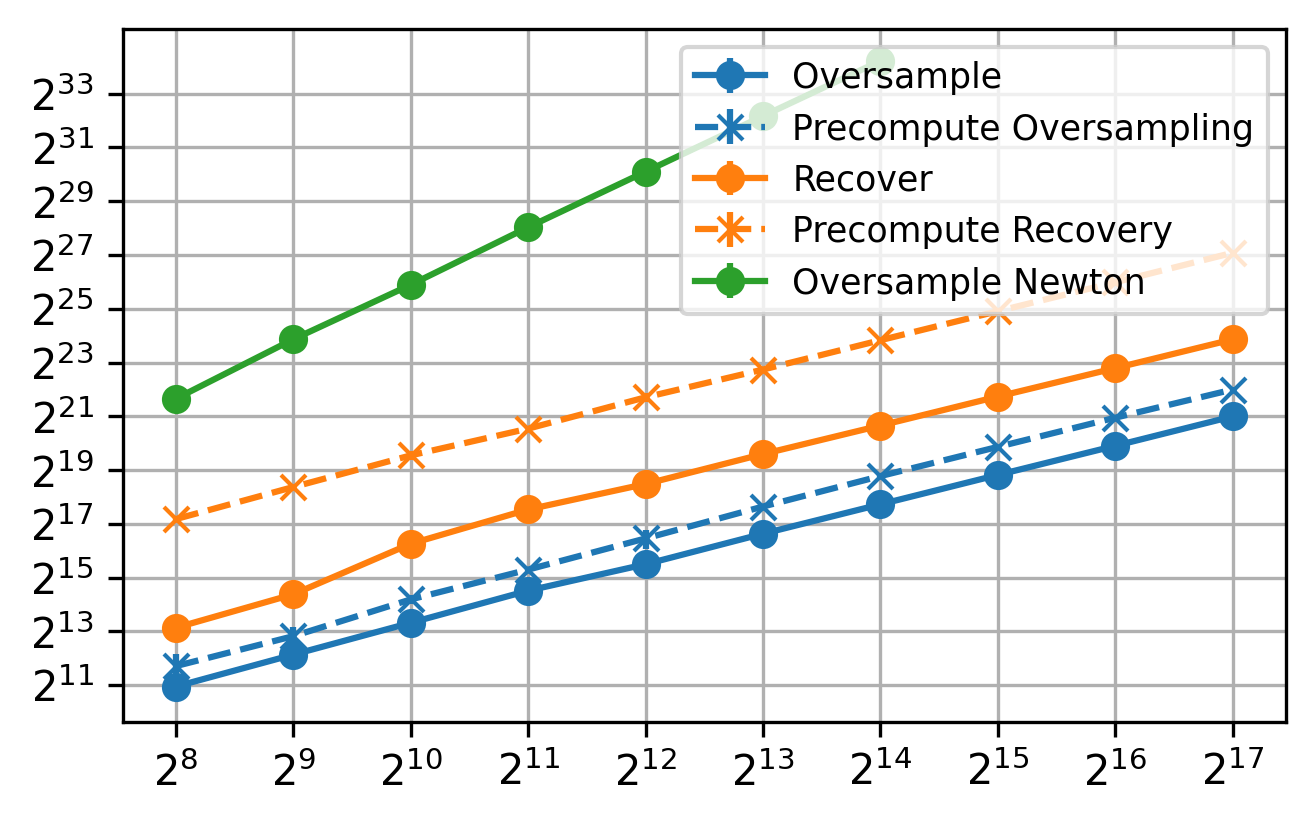
\includegraphics[width=0.9\textwidth]{benchmarks_log_poly.png}
\end{center}
\end{figure}

\end{frame}

\section{Conclusion}
\begin{frame}
\frametitle{Conclusion}

\begin{itemize}
\item
This has been a short presentation of the theory and implementation behind the \texttt{rsarc} file corruption repair utility, based on Reed-Solomon codes,
using transforms introduced in the paper "Novel Polynomial Basis and Its Application to Reed-Solomon Erasure Codes".

\item
Thank you for your time and attention!

\end{itemize}
\end{frame}

\end{document}
